% Created 2022-09-16 ven. 16:16
% Intended LaTeX compiler: pdflatex
\documentclass[10pt,table,dvipsnames,compress]{beamer}
\usepackage[utf8]{inputenc}
\usepackage[T1]{fontenc}
\usepackage{graphicx}
\usepackage{longtable}
\usepackage{wrapfig}
\usepackage{rotating}
\usepackage[normalem]{ulem}
\usepackage{amsmath}
\usepackage{amssymb}
\usepackage{capt-of}
\usepackage{hyperref}
\usetheme{default}
\useinnertheme{rounded}
\useoutertheme[subsection=false]{miniframes}
\date{}
\title{Computing the annual deforestation rate}
\title[Annual deforestation rate]{Computing the annual deforestation rate}
\usepackage{lmodern}
\usepackage{pgf}
\usepackage{color}
\usepackage[english,french]{babel}
\definecolor{vertmoyen}{RGB}{51,110,23} % vert moyen
\definecolor{blueFRB}{HTML}{31859c}
\usecolortheme[named=blueFRB]{structure}
\usepackage{tabularx} % varier la largeur du tableau
\usepackage{layout}
\setlength{\LTleft}{-5cm plus 1 fill}
\setlength{\LTright}{-5cm plus 1 fill}
\usepackage{booktabs}
\usepackage{arydshln} %% dashlines for tabular
\newcommand{\logit}{\text{logit}}
\newcommand{\bs}[1]{\boldsymbol{#1}}
\newcommand{\R}{\textnormal{\sffamily\bfseries R}}
\newcommand{\pkg}[1]{{\fontseries{b}\selectfont #1}}
\newcolumntype{C}[1]{>{\centering\arraybackslash}m{#1}}

\setbeamertemplate{footline}[frame number]
\setbeamertemplate{frametitle}{%
\usebeamerfont{frametitle}\insertframetitle%
\vphantom{g} % To avoid fluctuations per frame
\par
\centering 
\includegraphics[width=\textwidth]{figs/Barre_couleur}
}
\beamertemplatenavigationsymbolsempty

% Logo
\newif\ifplacelogo % create a new conditional
\logo{\ifplacelogo
\includegraphics[width=0.5\textwidth]{figs/partners_logos}\fi}

%Call table of contents at the beginning of each section
\AtBeginSection[]{
\placelogotrue
\begin{frame}
\frametitle{Plan}
\begin{columns}[c]
\begin{column}{0.5\textwidth}
\tableofcontents[sections=1,currentsection]
\vspace{0.5cm}
\tableofcontents[sections=2,currentsection]
\end{column}
\begin{column}{0.5\textwidth}
\tableofcontents[sections=3,currentsection]
\vspace{0.5cm}
\tableofcontents[sections=4,currentsection]
\end{column}
\end{columns}
\end{frame}
\placelogofalse
}

\AtBeginSubsection[]{}

\hypersetup{
colorlinks=true,
linkcolor=Black,
filecolor=Maroon,
citecolor=Blue,
urlcolor=Maroon}

% Disable monospaced font for URLs
\urlstyle{same}

\hypersetup{
 pdfauthor={Ghislain Vieilledent},
 pdftitle={Computing the annual deforestation rate},
 pdfkeywords={},
 pdfsubject={},
 pdfcreator={Emacs 27.1 (Org mode 9.5.3)}, 
 pdflang={English}}
\begin{document}


% Title page
{
  \setbeamertemplate{navigation symbols}{}
  \begin{frame}[plain, noframenumbering]
  
  \begin{center}
  \small{\textbf{Clark University -- JNR risk mapping meeting -- September 16th 2022}}
  \end{center}
  \vspace{-1cm}
  \titlepage % Presentation first page
  \vspace{-3.5cm}
  \begin{center}
    
\includegraphics[width=\textwidth]{figs/Barre_couleur}\\
    \vspace{0.5cm}
    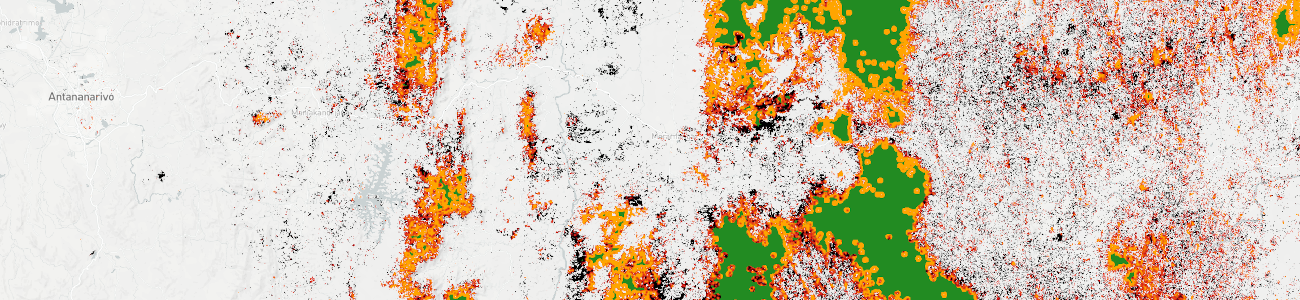
\includegraphics[width=10cm]{figs/riskmapjnr-example}\\
    \vspace{0.3cm}
    \small{Ghislain VIEILLEDENT$^{1}$\hspace{0.25cm}Pierrick RAMBAUD$^{2}$\hspace{0.25cm}Rémi d'ANNUNZIO$^{2}$}\\
    \vspace{0.15cm}
    {\scriptsize
      \begin{tabular}{l}
        $[1]$ \textbf{Cirad} UMR AMAP, $[2]$ \textbf{FAO} REDD$+$ NFM
      \end{tabular}
    }\\
    \vspace{0.3cm}
    
\includegraphics[width=0.75\textwidth]{figs/partners_logos}
    
  \end{center}
  \end{frame}
}

% %%%%%%%%%%%%%%%%%%%%%%%%%%%%%%%%%%%%%%%%%%%%%%%%%%%%%%%%%%%%%%%%

\placelogotrue
\begin{frame}
  \frametitle{Plan}
  \begin{columns}[c]
    \begin{column}{0.5\textwidth}
      \tableofcontents[sections=1]
      \vspace{0.5cm}
      \tableofcontents[sections=2]
    \end{column}
    \begin{column}{0.5\textwidth}
        \tableofcontents[sections=3]
        \vspace{0.5cm}
        \tableofcontents[sections=4]
    \end{column}
  \end{columns}
\end{frame}
\placelogofalse

\section{Introduction}
\label{sec:orgb4c6303}

\subsection{Context}
\label{sec:org55c81ef}

\begin{frame}[label={sec:org367d2e1}]{Observations of deforestation}
\begin{itemize}
\item Historical deforestation maps are often derived from the analysis of satellite images (eg. Landsat).
\item Deforestation is a rare event (< 1\%/yr) and is very variable from one year to another.
\item Deforestation is often observed and estimated for a period of time \(T\) of several years (eg. 5 or 10 years).
\end{itemize}

\begin{figure}[htbp]
\centering
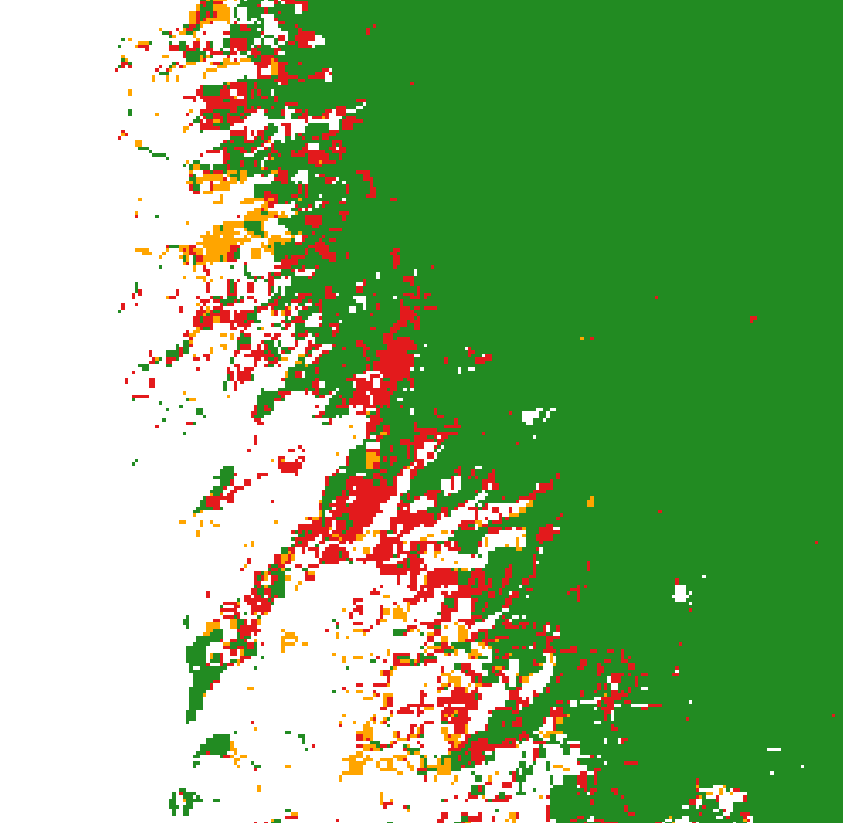
\includegraphics[width=0.35\textwidth]{figs/fcc123_zoom.png}
\caption{Deforestation 2000--2010--2020 in Guadeloupe.}
\end{figure}
\end{frame}

\begin{frame}[label={sec:orgb5e0994}]{Annual deforestation rate}
\begin{itemize}
\item To be able to compare deforestation intensity between regions (eg. countries) and time periods of different lengths (eg. 5 or 10 years), we need to compute a \alert{\alert{mean annual deforestation rate}} \(d\) in \%/yr (also denoted \%.yr\(^{-1}\)).
\item Several formulas have been proposed to compute \(d\) from the observed deforestation rate \(d'\) on a given period of time \(T\).
\item \(d' = (A_0-A_T)/A_0\), with \(A_0\): initial forest cover at time \(t=0\), and \(A_T\): forest cover at time \(t=T\) with \(T > 1\).
\end{itemize}
\end{frame}

\subsection{Objectives}
\label{sec:orgf827fb6}

\begin{frame}[label={sec:org3915a96}]{Objectives}
\begin{itemize}
\item Compare the different formulas used to compute the \alert{\alert{mean annual deforestation rate}} \(d\) in \%/yr.
\item Propose an appropriate formula for the JNR risk mapping tool.
\end{itemize}
\end{frame}

\section{Formulas}
\label{sec:orgcabe509}

\subsection{Notations}
\label{sec:org70b2c76}

\begin{frame}[label={sec:org450a6e4}]{Notations}
\begin{block}{Areas and time}
\begin{itemize}
\item \(A_t\): forest area (in ha or km\(^2\)) at time \(t\) with \(t=0,\ldots,T\).
\item \(A_0 > A_1 > A_2 > \ldots > A_T\).
\item \(T\): time-interval (in yr), \(T > 1\).
\end{itemize}
\end{block}

\begin{block}{Deforestation \alert{\alert{rates}}}
\begin{itemize}
\item \(d'\): observed deforestation rate for period of time \(T\). \\
\(d' = (A_0-A_T)/A_0\), in \%.
\item \(d\): \alert{\alert{mean annual deforestation rate}} over the period of time \(T\). \\
e.g. \(d=(A_0-A_1)/A_0\), in \%/yr.
\item \(d\) must be constant over the period of time \(T\). \\
\(d=(A_0-A_1)/A_0=(A_1-A_2)/A_1=\ldots_{}\).
\end{itemize}
\end{block}
\end{frame}

\subsection{Formulas}
\label{sec:org2aa6abd}

\begin{frame}[label={sec:org0c09095}]{Formulas}
How to compute \(d\) from \(A_0\), \(A_T\) and \(T\) (or from \(d'\) and \(T\) as \(d' = (A_0-A_T)/A_0\))?

\begin{block}{Proposed formulas}
\begin{itemize}
\item FAO formula \\
\(r = (A_T/A_0)^{(1/T)}-1\)
\item Clark U. formula (inverted ratio) \\
\(\delta = (A_0/A_T)^{(1/T)}-1\) \\
\item Puyravaud formula \\
\(\rho = (1/T) \ln(A_T/A_0)\)
\item Cirad formula (after correction)\\
\(d = 1 - (1 - d')^{1/T}\)
\end{itemize}
\end{block}
\end{frame}

\section{Formula comparison}
\label{sec:org1ae6ef4}

\subsection{FAO formula}
\label{sec:orgc295dbc}

\begin{frame}[label={sec:org4ae5568}]{FAO formula}
\centering \alert{\alert{\(r = (A_T/A_0)^{(1/T)}-1\)}}
\vspace{0.5cm}

\begin{itemize}
\item Following FAO definition, \(r\) is a mean \alert{\alert{annual rate of change}}, not a mean annual rate of \alert{\alert{deforestation}}.
\item This rate is zero if \(A_T = A_0\) (no change), positive if \(A_T > A_0\) (increase in forest cover), and negative if \(A_T <= A_0\) (deforestation). This equation is perfectly OK when correctly interpreted.
\item In the Verra document about JNR mapping risk methodology, there is a misinterpretation of \(r\) described as the deforestation or forest degradation rate (see p. 8 of the document).
\item To obtain a deforestation rate (which is assumed positive), we need the opposite:\\
\(d = 1 - (A_T/A_0)^{1/T}\)
\end{itemize}
\end{frame}

\subsection{Cirad formula}
\label{sec:orgccb075a}

\begin{frame}[label={sec:org9a7a8e3},fragile]{Cirad formula}
 \centering \alert{\alert{\(d = 1 - (1 - d')^{1/T}\)}}, with \(d' = (A_0-A_T)/A_0\) \\
\(d = 1 - (1 - (A_0-A_T)/A_0)^{1/T} = 1 - (A_T/A_0)^{1/T}\)
\vspace{0.5cm}

\begin{itemize}
\item This formula is just the \alert{\alert{opposite}} of the FAO rate cited by Verra:\\
\(d = 1 - r\), with \(r = (A_T/A_0)^{(1/T)}-1\).
\item Can be easily demonstrated mathematically.
\item Note that \(d = 1 - (1 - d')^{1/T} \Leftrightarrow d' = 1 - (1 - d)^{T}\)
\item This explains the error in the \texttt{riskmapjnr} Python package (there was a confusion between \(d\) and \(d'\), now corrected).
\end{itemize}
\end{frame}

\subsection{Clark U. formula}
\label{sec:orga8241e4}

\begin{frame}[label={sec:orgde71943}]{Clark U. formula}
\centering \alert{\alert{\(\delta = (A_0/A_T)^{(1/T)}-1\)}}
\vspace{0.25cm}

\begin{columns}
\begin{column}{0.5\columnwidth}
\begin{itemize}
\item Inverse ratio \(A_0/A_T\) in place of \(A_T/A_0\).
\item Seems to provide reasonable estimates.
\end{itemize}
\end{column}

\begin{column}{0.5\columnwidth}
\begin{center}
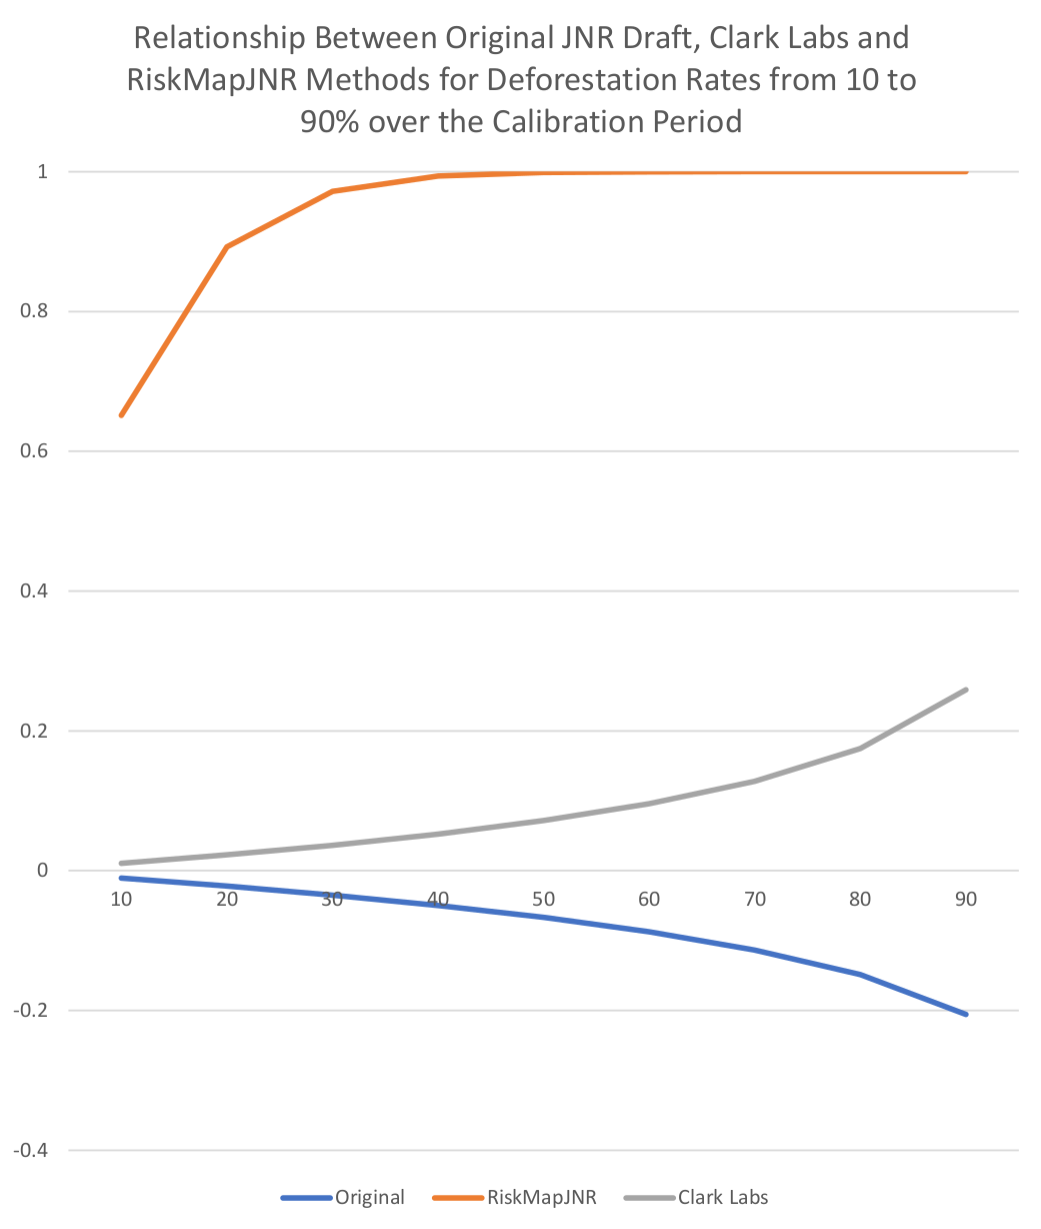
\includegraphics[width=\textwidth]{figs/clarku.png}
\end{center}
\end{column}
\end{columns}
\end{frame}

\begin{frame}[label={sec:orgba525dd}]{Problems with Clark U. formula}
\centering \alert{\alert{\(\delta = (A_0/A_T)^{(1/T)}-1\)}}
\vspace{0.25cm}

\begin{itemize}
\item Not defined when \(A_T=0\)
\item \(A_T=0\) is frequent (small window size or \(T\) is large).
\item Difficult to interpret.
\item Overestimation of the mean annual deforestation rate.
\end{itemize}

\begin{center}
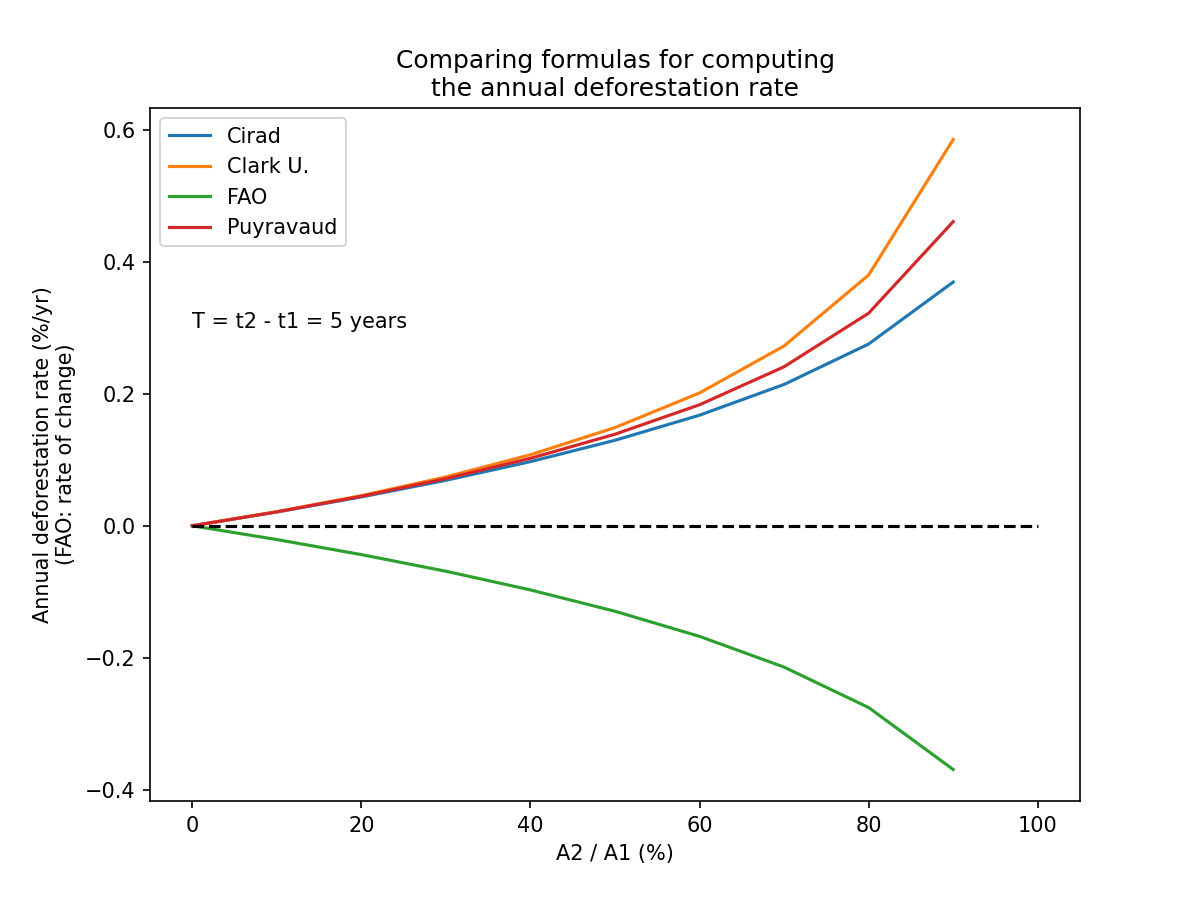
\includegraphics[width=0.6\textwidth]{figs/D-perc-relationship.png}
\end{center}
\end{frame}

\begin{frame}[label={sec:org558f892}]{Problems with Clark U. formula}
\centering \alert{\alert{\(\delta = (A_0/A_T)^{(1/T)}-1\)}}
\vspace{0.25cm}

\begin{itemize}
\item Overestimation of the mean annual deforestation rate.
\end{itemize}

\begin{center}
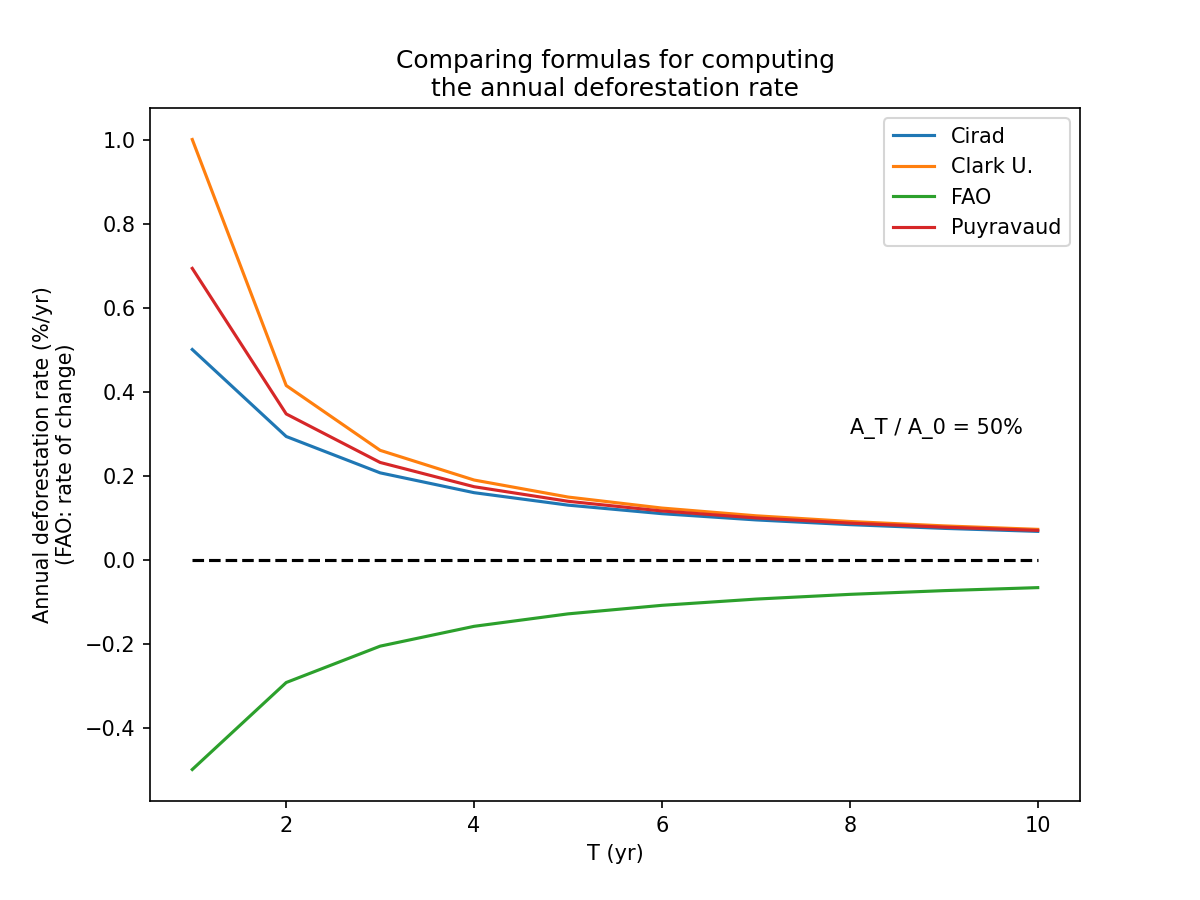
\includegraphics[width=0.6\textwidth]{figs/D-T-relationship.png}
\end{center}
\end{frame}

\subsection{Puyravaud formula}
\label{sec:orgb93642b}

\begin{frame}[label={sec:org06c39d0}]{Puyravaud formula}
\centering \alert{\alert{\(\rho = (1/T) \ln(A_T/A_0)\)}}
\vspace{0.25cm}

\begin{itemize}
\item Derived from the instantaneous rate of change.
\item Not defined when \(A_T=0\).
\item Again, \(A_T=0\) is frequent (small window size or \(T\) is large).
\item Overestimation of the mean annual deforestation rate.
\end{itemize}

\begin{columns}
\begin{column}{0.5\columnwidth}
\begin{center}
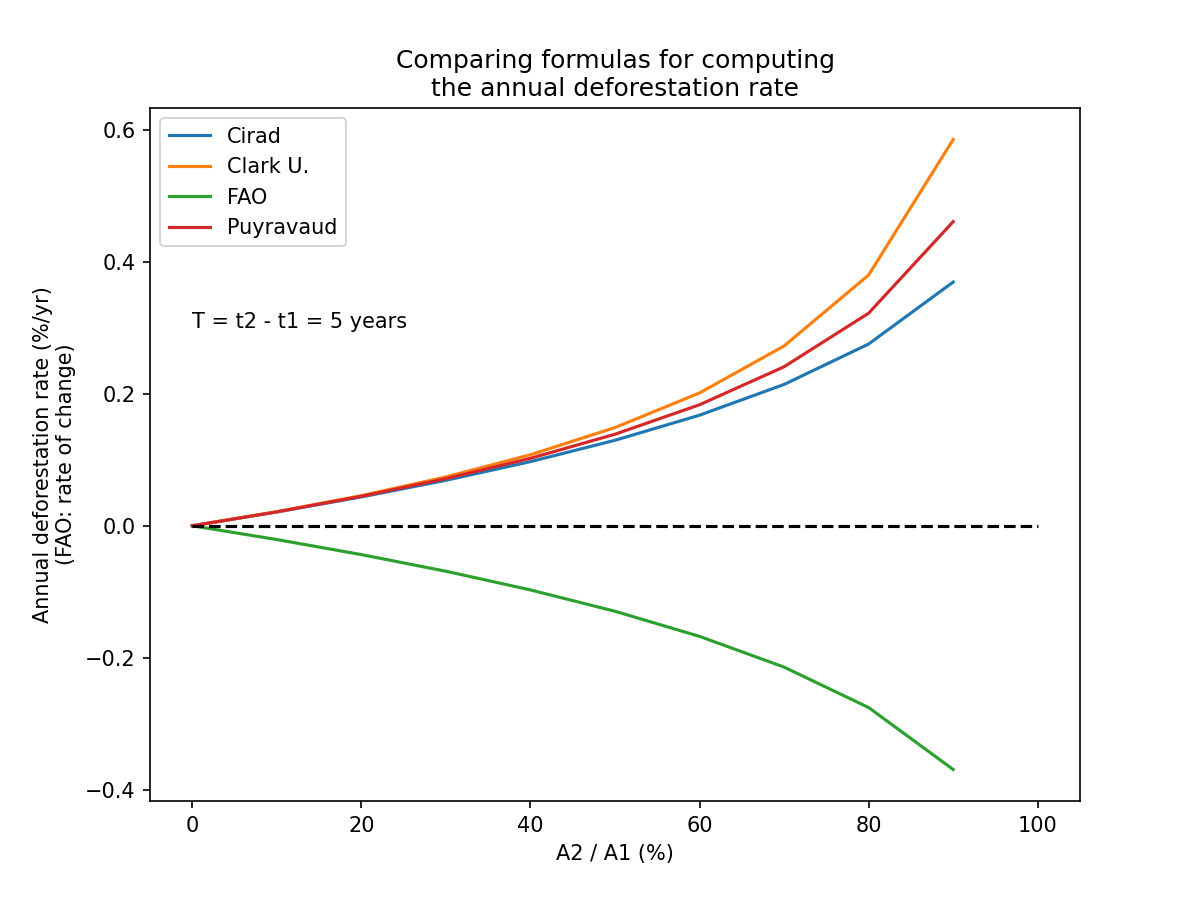
\includegraphics[width=\textwidth]{figs/D-perc-relationship.png}
\end{center}
\end{column}

\begin{column}{0.5\columnwidth}
\begin{center}
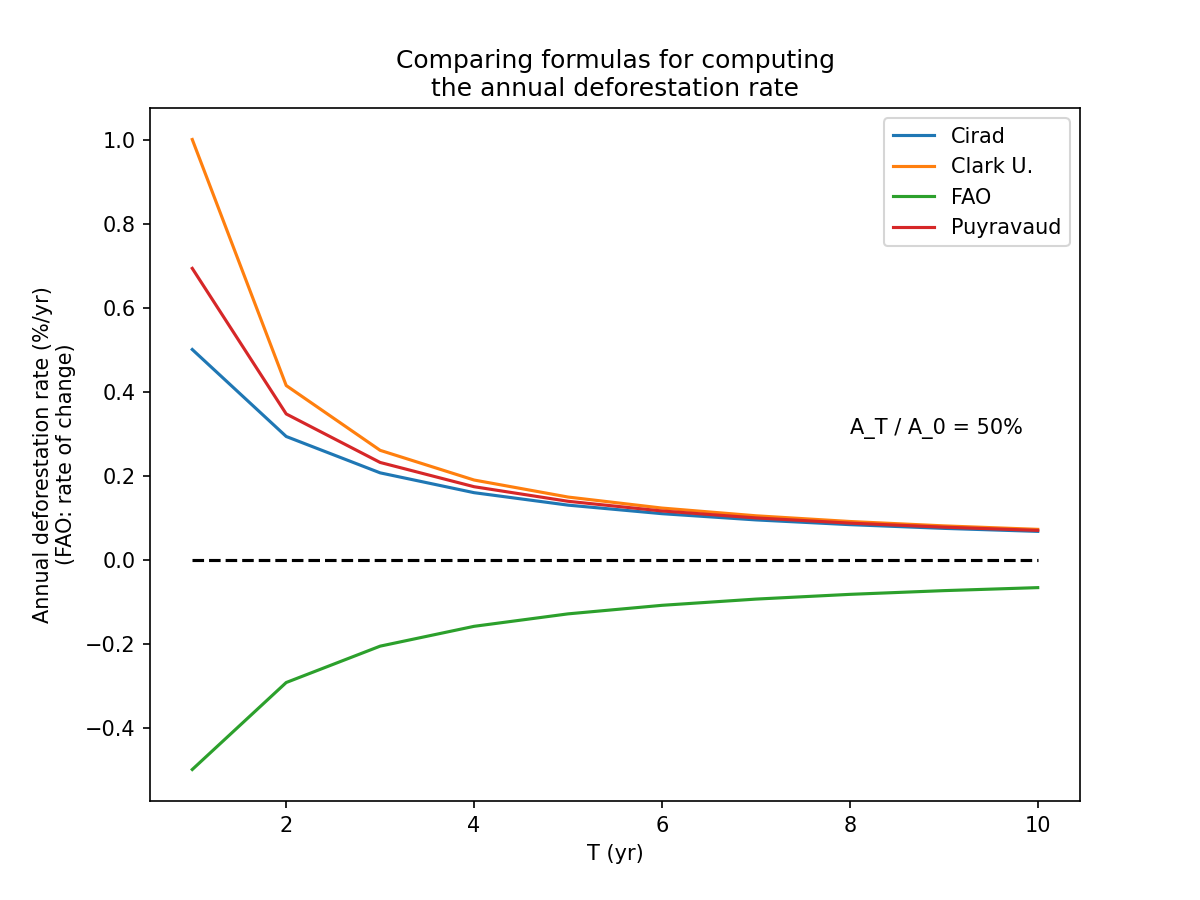
\includegraphics[width=\textwidth]{figs/D-T-relationship.png}
\end{center}
\end{column}
\end{columns}
\end{frame}

\section{Conclusion}
\label{sec:orgf3a85e5}

\subsection{Recommendation}
\label{sec:org3b3e10a}

\begin{frame}[label={sec:org82a0c1c}]{Recommendation}
We recommend the use of the following formula to estimate the \alert{\alert{mean annual deforestation rate}}:\\
\vspace{0.25cm}

\centering \alert{\alert{\(d = 1 - (1 - d')^{1/T}\)}} equivalent to \alert{\alert{\(d = 1 - (A_T/A_0)^{1/T}\)}}
\end{frame}

\subsection{Demonstration of the formula}
\label{sec:orgb888852}

\begin{frame}[label={sec:org314c2f9}]{Demonstration}
We demonstrate that \alert{\alert{\(d = 1 - (1 - d')^{1/T}\)}}: \\
\vspace{0.25cm}

We have: \(A_0 > A_1 > A_2 > \ldots > A_T\) \\
Then, \(A_1 = A_0 - d \times A_0 = A_0 (1-d)\) \\
\(A_2 = A_1 - d \times A_1 = A_1 (1-d) = A_0 (1-d) (1-d) = A_0 (1-d)^2\) \\
\(\ldots\) \\
\(A_T = A_0 (1-d)^T\) \(\Leftrightarrow\) A\textsubscript{T}/A\textsubscript{0}=(1-d)\textsuperscript{T} \alert{\alert{(1)}} \\
\vspace{0.25cm}

By definition, d'=(A\textsubscript{0}-A\textsubscript{T})/A\textsubscript{0} \alert{\alert{(2)}} \\
\vspace{0.25cm}

\alert{\alert{(1)}} and \alert{\alert{(2)}} \(\Rightarrow\) \(d' = 1 - (1-d)^T\) \alert{\alert{(3)}} \\
\((1-d)^T = 1-d'\) \\
\(1-d = (1-d')^{1/T}\) \\
\alert{\alert{\(d = 1 - (1 - d')^{1/T}\) (4)}}
\end{frame}

% %%%%%%%%%%%%%%%%%%%%%%%%%%%%%%%%%%%%%%%%%%%%%%%%%%%%%%%%%%

{
  % Use background image
  \usebackgroundtemplate{%
    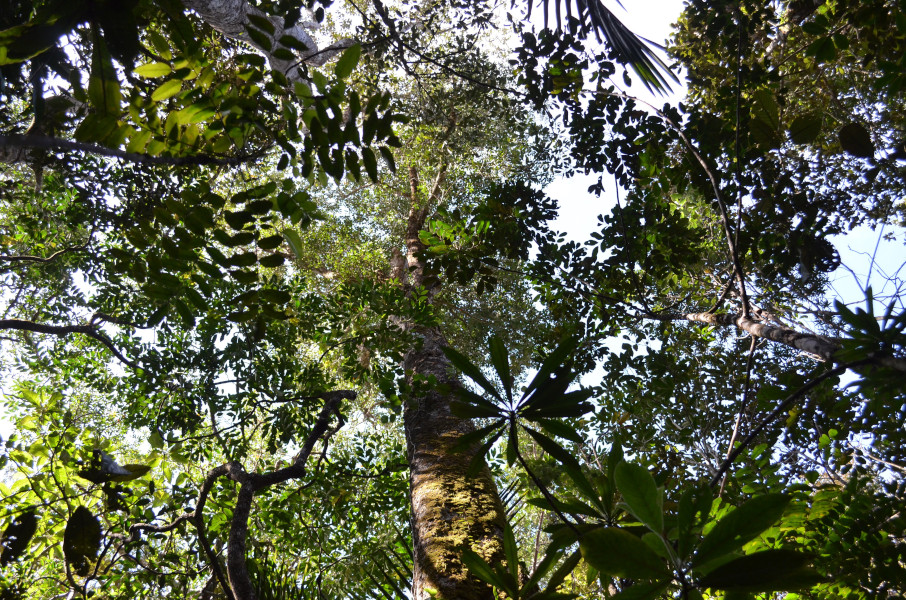
\includegraphics[keepaspectratio=true, height=\paperheight]{figs/Canopy-NC}
  }
  \setbeamertemplate{navigation symbols}{}
  % Remove shadow from block
  \setbeamertemplate{blocks}[rounded][shadow=false]
  \begin{frame}[plain]
  	\vspace*{\stretch{100}} 
    \begin{block}{}
      \begin{center}
        \ldots~Thank you for attention~\ldots \\
        \url{https://ecology.ghislainv.fr/presentations} \\
        
\includegraphics[width=0.45\textwidth]{figs/partners_logos}
      \end{center}
    \end{block}
  \end{frame}
}
\end{document}